\chapter{Aufbau}
\label{chap:aufbau}

Dieses Kapitel befasst sich mit dem Aufbau, welcher alle Sensoren und Aktuatoren miteinander verbindet.
Die erste Überlegung war, den beweglichen Teil als Pendel auszuführen.
Diese Idee ist zwar gut, allerdings ist das Pendel durch die Reibung von den Schleifringen für die Elektronik zu stark gebremst worden.
Dadurch musste mit dem Magneten, welcher das Pendel bei jedem Nulldurchgang beschleunigte, eine relativ große Kraft übertragen werden.
Das Problem an dieser Lösung war, dass das Pendel nicht mehr frei schwingt, sondern deutliche Unregelmäßigkeiten beobachtet werden können.
Als Lösung wurde der Entwurf mit dem Pendel überarbeitet und es wurde stattdessen eine Scheibe verwendet.
Der Antrieb erfolgt durch einen Schrittmotor, dadurch kann eine vorgegebene Drehgeschwindigkeit eingestellt werden.
Ein weiterer Vorteil ist, dass die vorgegebene Geschwindigkeit sehr konstant gehalten werden kann.
Dieser Aufbau wird in Abbildung~\ref{fig:3dSchreibe} dargestellt.
In dieser 3D-Zeichnung kann man auch die Lichtschranken für den Drehgeber, die Schrittmotoren für die Spiegel und deren Lichtschranken erkennen.

\begin{figure}[!h] \centering
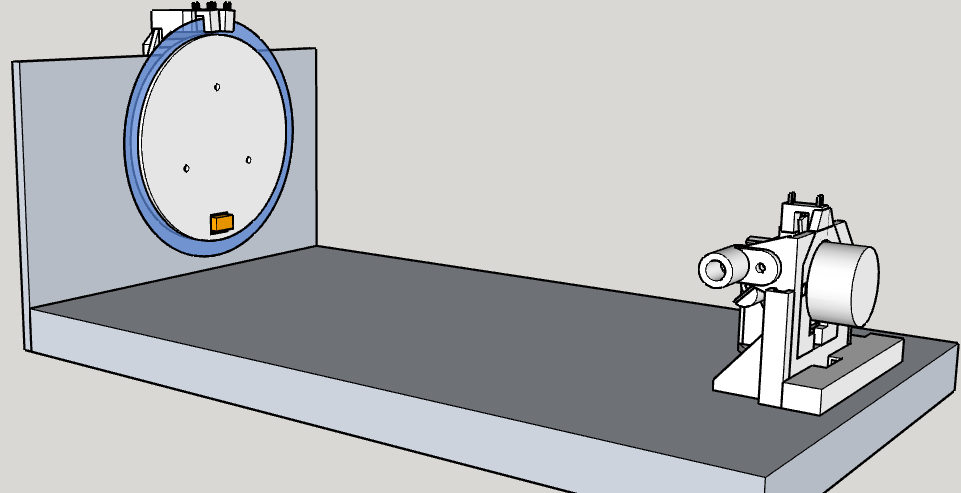
\includegraphics[width=0.7\textwidth]{img/Sketchup/Disc00.PNG}
\caption{3D-Modell des Prototypen.}
\label{fig:3dSchreibe}
\end{figure}


\section{Spiegelablenkeinheit}
Die Berechnung der Winkel für die Spiegel wird für die Studenten, welche mit diesem Modell arbeiten werden, ein Kernpunkt.
Natürlich müssen die maximalen Winkel, welche mit eingeschaltetem Laser erreicht werden dürfen, bereits vorher bekannt sein.
Im folgenden wird näher darauf eingegangen.

\subsection{Berechnung der Winkel}
\begin{figure}[!h] \centering
	\begin{tikzpicture}[scale=1.5]
\pgfmathsetmacro\VarGamma{35};
\pgfmathsetmacro\VarCosAlpha{cos(90-\VarGamma*2)};
\pgfmathsetmacro\VarSinAlpha{sin(90-\VarGamma*2)};

\coordinate (N) at (90-\VarGamma:2);
\coordinate (O) at (0,0);
\coordinate (E) at (90:3);
\coordinate (Y) at (90:4);
\coordinate (X) at (0:4);
\coordinate (A) at (90-2*\VarGamma:3);
\coordinate (TU) at (3*\VarCosAlpha,0);
\coordinate (TO) at (3*\VarCosAlpha,3);
\coordinate (Ttxt) at (3*\VarCosAlpha,2*\VarSinAlpha);
\coordinate (Ctxt) at (2*\VarCosAlpha,0);

%Achsen zeichnen
\draw[thin,->] (-2,0) -- (X) node[right]{$x$};
\draw[thin,->] (0,-1) -- (Y) node[left]{$y$};
\draw[thick] (-\VarGamma:2) -- (-\VarGamma:-2);
\draw[very thick,->] (E) -- (O);
\draw[dashed] (O) -- (90-\VarGamma:4);
\draw[very thick,->] (O) -- (A);
\draw[thick] (TU) -- (TO);
\draw (Ttxt) node[right]{$a$};
\draw (Ctxt) node[below]{$b$};

\pic[draw=black,angle eccentricity=0.8,angle radius=1.5cm,pic text={$\gamma$}] {angle=N--O--E};
\pic[draw=black,angle eccentricity=0.8,angle radius=1.5cm,pic text={$\gamma$}] {angle=A--O--N};
\pic[draw=black,angle eccentricity=0.8,angle radius=1.5cm,pic text={$\alpha$}] {angle=X--O--A};
\end{tikzpicture}
	\caption{Winkel bei der Laserablenkeinheit.}
	\label{fig:angles}
\end{figure}

In Abbildung~\ref{fig:angles} sind die Winkel der Spiegelablenkeinheit dargestellt.
Hierbei sind die Laserstrahlen als dicke Linien und die Normale auf den Spiegel als strichlierte Linie dargestellt.
Dabei bezeichnet $\gamma$ den Winkel, welcher die Normale des Spiegels mit dem einfallenden Laserstrahl einschließt.
$\alpha$ bezeichnet den einschließenden Winkel zwischen dem Ausfallstrahl und der Grundplatte.
Diese Winkel können wie folgt berechnet werden.
\begin{equation}
\alpha=arctan(a/b)
\end{equation}
\begin{equation}
\gamma=\frac{90^\circ-\alpha}{2}
\end{equation}
Um zu berechnen wo der Laserstrahl auf die Wand projiziert wird, muss nur auf $a$ umgeformt werden.
\begin{equation} \label{equ:posOfLaser}
a=b \cdot tan(90^\circ-2 \cdot \gamma)
\end{equation}
Diese Überlegungen gelten sowohl für die horizontale als auch die vertikale Richtung.


\subsection{Marken für Endpositionen}

\begin{figure}[!h] \centering
	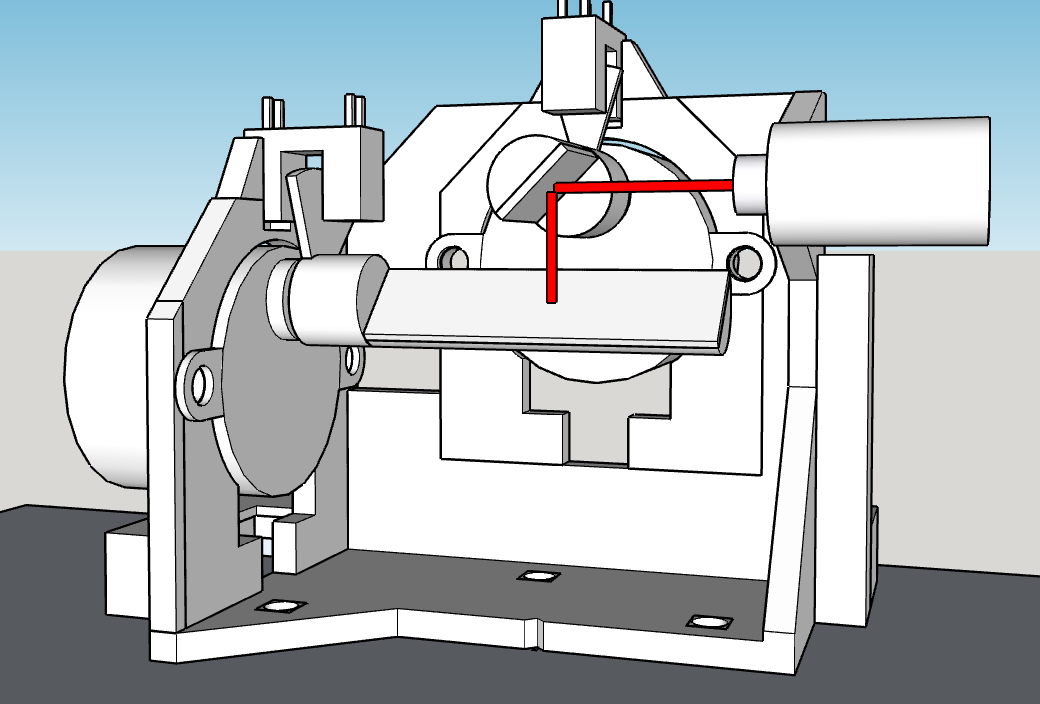
\includegraphics[width=0.7\textwidth]{img/Sketchup/Lasercontroll00.PNG}
	\caption{3D-Modell der Spiegelablenkeinheit.}
	\label{fig:laserablenkeinheit}
\end{figure}

Die Überlegungen, welche Winkel eingestellt werden müssen, sind nicht nur für die Positionierung des Lasers wichtig, sondern auch für die Berechnung der Bereichsmarken.
Diese Marken geben an, ob bei dieser Winkeleinstellung der Laserstrahl gefahrlos aktiviert werden kann.
Dies ist nur dann der Fall, wenn der Laserpunkt auf der Rückwand des Prototypen projiziert wird.
Dazu wird im Modell eine Markierung auf den Motoren angebracht, welche bei der maximalen Auslenkung einen Lichtschranken unterbricht.

Sei $a$ in dieser Überlegung die maximal erlaubte Auslenkung auf der Projektionsfläche, welche gefahrlos eingestellt werden darf.
Zusätzlich nehmen wir an, dass die Lichtschranken entlang des einfallenden Lasers positioniert sind.
Das bedeutet, dass der Laser abgeschaltet wird, sobald eine gedachte Marke in Abbildung~\ref{fig:angles} die y Achse überschreitet.
Diese Marke ist winkelfest mit der strichlierten Normale und dem Spiegel verbunden.
Unter diesen Voraussetzungen gibt $\gamma$ den Winkel an, mit welchem die Marke konstruiert werden muss.
Dieser Winkel reicht von dem Ende der Marke bis zur Normale des Spiegels.
Das 3D-Modell der fertigen Konstruktion ist in Abbildung~\ref{fig:laserablenkeinheit} ersichtlich.



\section{Inkrementalgeber}

\subsection{Funktionsweise}

\begin{figure}[!h] \centering
	\begin{minipage}[t]{.49\linewidth} \centering
		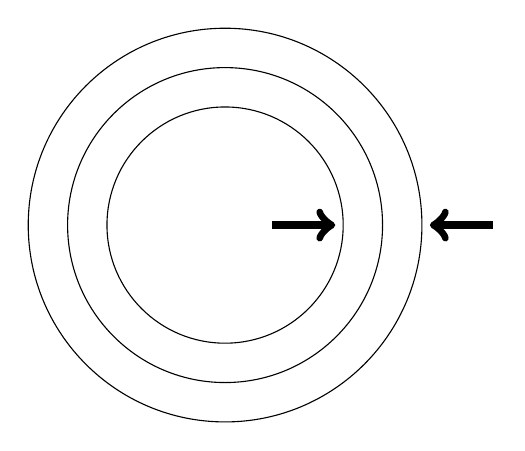
\begin{tikzpicture}
\pgfmathsetmacro{\scale}{2.5}
\pgfmathsetmacro{\parts}{5}
\pgfmathsetmacro{\posOut}{1}
\pgfmathsetmacro{\posMiddle}{0.8}
\pgfmathsetmacro{\posIns}{0.6}

\pgfmathsetmacro{\circles}{\parts*4}
\pgfmathsetmacro{\posOut}{1 * \scale}
\pgfmathsetmacro{\posMiddle}{0.8 * \scale}
\pgfmathsetmacro{\posInside}{0.6 * \scale}
\pgfmathsetmacro{\partAngle}{360 / \circles}
\path (0,0)[draw=black] circle (\posOut);
\path (0,0)[draw=black] circle (\posMiddle);
\path (0,0)[draw=black] circle (\posInside);
\foreach\i in {0,4,...,\circles} {
    \drawStrip{black}{\partAngle}{\i + 0}{\posMiddle}{\posOut}
    \drawStrip{black}{\partAngle}{\i + 1}{\posMiddle}{\posOut}
    \drawStrip{black}{\partAngle}{\i + 1}{\posInside}{\posMiddle}
    \drawStrip{black}{\partAngle}{\i + 2}{\posInside}{\posMiddle}
}
\draw [black,<-,line width=3pt] ({\posInside - 0.1},0) -- +(-0.8,0);
\draw [black,<-,line width=3pt] ({\posOut + 0.1},0) -- +(0.8,0);
\end{tikzpicture}

	\end{minipage}
	\begin{minipage}[t]{.49\linewidth} \centering
		%position, label
\newcommand*{\drawSingleQuadratureDiagram}[1]{
	\tikzstyle{line}=[color=black,line width=1.5pt]
	\draw(0,1) node[left]{1};
	\draw(0,0) node[left]{0};
	\begin{scope}[shift={({0.5 * (#1)},0 )}]
		\drawSquarewave{line}{2}{1}{1}{1}{1}
	\end{scope}
}

\begin{tikzpicture}
	\drawSingleQuadratureDiagram{0}
	\begin{scope}[shift={(0,1.5 )}]
	\drawSingleQuadratureDiagram{1}
	\end{scope}
\end{tikzpicture}

	\end{minipage}
	\caption{Funktionsweise eines Drehgebers.}
	\label{fig:drehgeber}
\end{figure}

Ziel eines Drehgebers ist es, die Position der Scheibe zu ermitteln.
Je nach Aufgabenstellung gibt es dazu verschiedene Arten von Drehgebern.
Grundsätzlich wird zwischen Absolutgebern und Inkrementalgebern unterschieden.
Erstere haben auf der Scheibe, welche in n Segmente unterteilt ist, genau $log_2(n)$ Spuren mit einem Binärcode.
Jede Spur wird mit einem separaten Sensor ausgewertet.
Dadurch kann immer ausgelesen werden, in welchem Segment sich die Leseköpfe der Sensoren befinden.

Nachteilig an einen Absolutgeber ist, dass eine hohe Anzahl an Sensoren und auch an Spuren auf der Scheibe benötigt wird.
Dadurch ist er für dieses Projekt nicht von Bedeutung, da für eine annehmbare Schrittauflösung zu viele Sensoren verwendet werden müssten.

Bei einem Inkrementalgeber kann man die Anzahl der Sensoren reduzieren, indem man nur zwei Bahnen verwendet, welche je ein Rechtecksignal produzieren.
Die beiden Rechtecksignale sind zueinander eine Viertelperiode versetzt.
Eine andere Variante, welche noch einfacher realisierbar ist, ist nur eine Spur zu verwenden und stattdessen die Sensoren um eine Viertelperiode voneinander versetzt anzuordnen.
Eine Illustration einer solchen Abnehmerkonstellation ist in Abbildung~\ref{fig:drehgeber} dargestellt. \cite[333]{book:elektrischeMesstechnik}

\begin{figure}[!h] \centering
	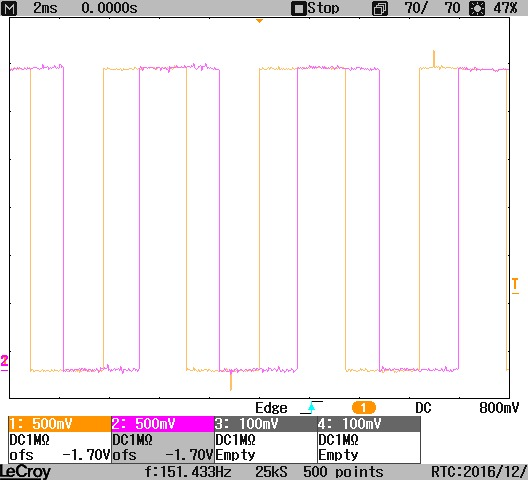
\includegraphics[width=0.7\textwidth]{img/PicturesPlots/Encoder/Normal/COPY/CONVERT/SCRN0117_Cutted.jpg}
	\caption{Aufnahme des Quadratursignals der drehbaren Scheibe.}
	\label{fig:quadratureSignalNormal}
\end{figure}

Das Ausgangssignal hat nun die Form eines 2-Bit-Gray-Codes.
Wenn nun das Signal ausgewertet wird, kann bei jeder Flanke die Richtung des Schrittes ermittelt werden.
In Abbildung~\ref{fig:quadratureSignalNormal} ist eine Aufnahme, des von diesem Prototypen produzierten Signals, abgebildet.


\subsection{Betrachtung durch endliche Automaten}
\label{chap:aufbau:aufbauInkrementalgeberFSM}

\begin{figure}[!h] \centering
	\begin{minipage}[t]{.5\linewidth} \centering
		\begin{tikzpicture}[->,>=stealth',shorten >=1pt,auto,node distance=3cm,
  thick,main node/.style={circle,fill=blue!20,draw,font=\sffamily\Large\bfseries}]

  \node[main node] (1) {0 0};
  \node[main node] (2) [below left of=1] {0 1};
  \node[main node] (3) [below right of=2] {1 1};
  \node[main node] (4) [below right of=1] {1 0};

  \path[every node/.style={font=\sffamily\small}]
(1) edge 				node [left] 	{F} (4)
(1) edge [bend right] 	node[left] 	{B} (2)
(2) edge 				node [right] 	{F} (1)
(2) edge [bend right] 	node[left] 	{B} (3)
(3) edge 				node [right]	{F} (2)
(3) edge [bend right] 	node[right] 	{B} (4)
(4) edge 				node [left]	{F} (3)
(4) edge [bend right] 	node[right] 	{B} (1);
\end{tikzpicture}
	\end{minipage}
	\caption{FSM eines Drehgebers.}
	\label{fig:drehgeberZustaende}
\end{figure}

Eine einfache Betrachtungsweise, welche sehr elegant in Software implementiert werden kann, ist die Darstellung durch einen endlichen Automaten, auch Zustandsmaschine oder Finite-State-Machine (FSM) genannt.
Dabei gibt es vier Zustände und jeder stellt eine Kombination der beiden Eingänge dar.
Ein Zustandswechsel wird durch einen logischen Wechsel eines Einganges ausgelöst und gibt als Ausgabe entweder einen Vorwärts- oder einen Rückwärtsschritt zurück.
Um die Gesamtposition zu errechnen müssen nur alle Schritte vorzeichenrichtig gezählt werden.

Eine FSM, welcher den geschilderten Sachverhalt implementiert, ist in Abbildung~\ref{fig:drehgeberZustaende} dargestellt.
Damit die abgebildete Graphik eine gültige FSM wird, müssen noch Anfangszustand und gültige Endzustände eingezeichnet werden.
Der Anfangszustand ergibt sich jedoch daraus, wie die Encoderscheibe bei der Initialisierung des Controllers steht und kann deswegen noch nicht eingezeichnet werden.
Der Endzustand ist der letzte eingelesene Zustand. \cite[51]{book:evolvableSystems}


\subsection{Fehlerquellen}

Bei dieser Variante gibt es allerdings bestimmte Eigenschaften, welche bei der Implementierung berücksichtigt werden müssen.
Da dies nur eine inkrementelle Positionierung ist, ist der Startpunkt nicht durch das Sensorsignal ermittelbar.
Weiteres werden einmalige Fehler aufaddiert und können nur mit dem Rotationsencoder nicht mehr korrigiert werden.
Da bei Inkrementalgebern mit hoher Schrittauflösung sehr viele Wechsel von Flanken verarbeitet werden müssen, können bei hohen Drehgeschwindigkeiten Schritte verloren gehen.
Selbst eine sehr effiziente Implementierung mit Interrupts ist nicht für jeden Inkrementalgeber ausreichend.
Abhilfe schafft in diesem Fall nur die Verwendung eines Mikrocontrollers mit einem eingebauten Quadraturencoder oder einer speziellen zusätzlichen Hardware.


\subsection{Nulldurchgangsdetektion mit großer Schrittmarke}
\label{chap:aufbau:bigMark}

Um ohne zusätzliche Sensoren den Nulldurchgang detektieren zu können, können in die Encoderscheibe zusätzliche Information eingefügt werden.
Eine Variante ist, dass ein einziger Puls mit dreifacher Länge eingefügt wird.
Dadurch ist ein Nulldurchgang erkennbar.
Allerdings verliert man dadurch die Möglichkeit, schnelle Richtungswechsel detektieren zu können.
Nimmt man nun an, dass die Anzahl an Richtungswechsel sehr klein im Vergleich zu den Umdrehungen sind, kann man durch diese Zusatzinformation sowohl die Drehrichtung als auch die Nulldurchgänge erkennen.
Für diesen Prototypen wurde eine Marke mit der dreifachen Länge verwendet.
Dies ist gleich einem ausgefüllten Zwischenraum der Encoder-Scheibe.

\begin{figure}[!h] \centering
	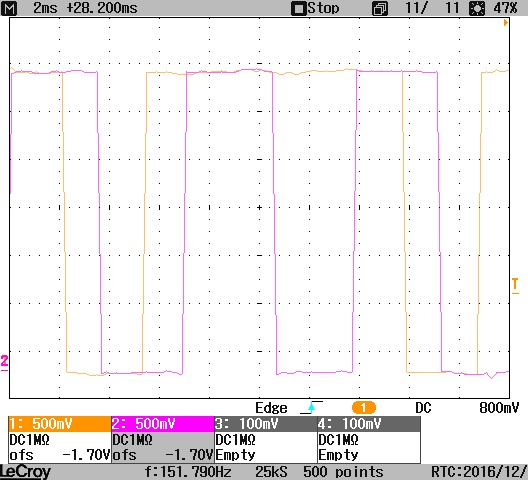
\includegraphics[width=0.7\textwidth]{img/PicturesPlots/Encoder/BigStep/COPY/CONVERT/SCRN0110_Cutted.jpg}
	\caption{Aufnahme des Quadratursignals der drehbaren Scheibe.}
	\label{fig:quadratureSignalBig}
\end{figure}

Eine Aufnahme des Signals bei einer großen Marke ist in Abbildung~\ref{fig:quadratureSignalBig} abgebildet.
Wenn diese Schrittkombination mit der in Kapitel~\ref{chap:aufbau:aufbauInkrementalgeberFSM} erläuterten FSM abgearbeitet wird, kann die Marke dadurch erkannt werden, dass genau ein Schritt in die falsche Richtung generiert wird.
Dies zu erkennen ist trivial.
Wichtig ist noch anzumerken, dass diese Marke doppelt auftritt, für jeden Sensor einmal.
Als Nullpunkt darf aber nur eine der beiden Stellen verwendet werden.
Für eine korrekte Funktionsweise ist zusätzlich ein ausreichend großer Schrittabstand zwischen den beiden aufnehmenden Sensoren nötig.

Nun müssen allerdings die Schritte, welche durch dieses neue Muster verloren gegangen sind, durch virtuelle Schritte ersetzt werden.
Bei jeder Detektion einer großen Marke wird nun ein Rückwärtsschritt statt einem Vorwärtsschritt detektiert und es gehen aufgrund der fehlenden Flanken zwei Pulse verloren.
Daher müssen bei jeder der beiden Detektionen des breiten Impulses vier Impulse addiert werden.
Nur bei einem der beiden darf die aktuelle Schrittzahl auf Null gesetzt werden.


\subsection{Beispielscheibe für Inkrementalgeber}

\begin{figure}[!h] \centering
	\newcommand{\drawArc}[4]{%Angle1,Angle2,Radius1,Radius2
	\draw[fill=black, line width=0mm]
	(#2:#3) arc
	(#2:#1:#3) --
	(#1:#4) arc
	(#1:#2:#4) --
	cycle;
}

\newcommand{\rotaryEncoderLines}[5]{%Angle1, Angle2, DegreeStep, Radius1, Radius2
	\pgfmathsetmacro{\angleSecond}{#1+#3*2};
	\foreach \a in {#1,\angleSecond,...,#2}
	{
		\drawArc{\a}{\a+#3}{#4}{#5};
	}
}

\newcommand{\drawSimpleRect}[2]{%sizeB sizeB
	\draw[line width=0.1mm] (#1,#2) -- (-#1,#2);
	\draw[line width=0.1mm] (-#1,#2) -- (-#1,-#2);
	\draw[line width=0.1mm] (-#1,-#2) -- (#1,-#2);
	\draw[line width=0.1mm] (#1,-#2) -- (#1,#2);
}

\newcommand{\rotaryEncoder}[4]{%OuterRadius, LineWidth, DetectorAngle, DetectorPulses
	\pgfmathsetmacro{\stepDegree}{2*#3/#4};
	\rotaryEncoderLines{0}{360}{\stepDegree}{#1-#2}{#1};
	\drawArc{\stepDegree}{2*\stepDegree}{#1-#2}{#1};
	\foreach \a in {0,120,240} {
		\draw (\a+90:25mm) circle (3mm);
		\draw (\a+90:25mm) circle (1.5mm);
	}
	\begin{scope}[shift={(0,-31mm)}]
		\drawSimpleRect{9mm}{16mm}
	\end{scope}
	\drawSimpleRect{5mm}{5mm}

	\pgfmathsetmacro{\pulses}{360/\stepDegree};
	\node[draw,rotate=0] (t) at (90:38mm) {Step-$\angle$: \stepDegree$^\circ$};
	\node[draw,rotate=30] (t) at (135:30mm) {Detector-$\Delta$-$\angle$: #3$^\circ$};
	\node[draw,rotate=-30] (t) at (45:30mm) {Detector-$\Delta$-$\sqcap$: #4};
	\node[draw,rotate=0] (t) at (90:15mm) {$\sqcap$: \pulses};
}

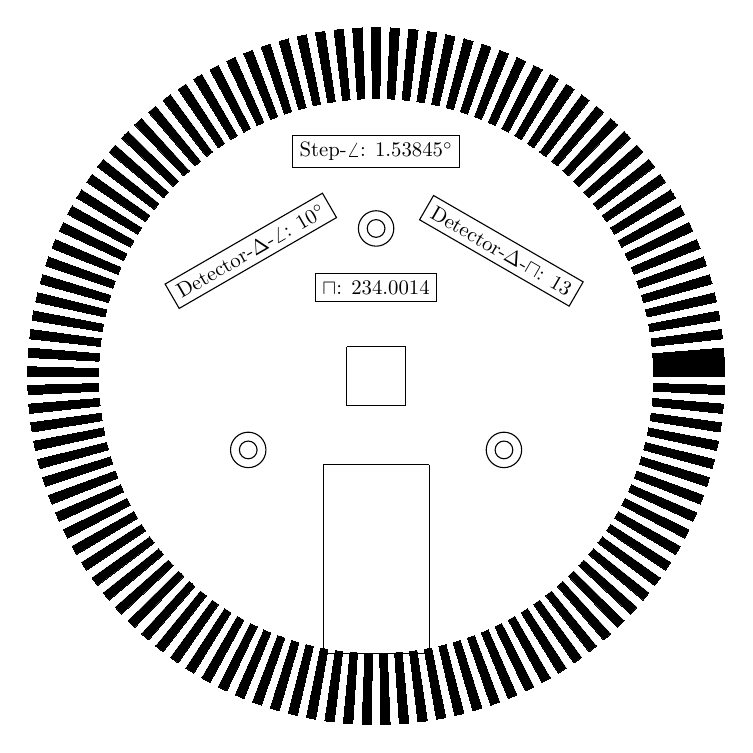
\begin{tikzpicture}[scale=0.75, transform shape]
\rotaryEncoder{59mm}{12mm}{10}{13}
\end{tikzpicture}


	\caption{Scheibe für den Rotationsencoder.}
	\label{fig:rotaryEncoderDisc}
\end{figure}

Die Scheibe für diesen Prototypen wurde mit Latex und Tikz gezeichnet.
Dabei wurde zum Testen ein Template erstellt, welches beliebig konfiguriert werden kann.
In Abbildung~\ref{fig:rotaryEncoderDisc} ist die verwendete Scheibe dargestellt.
Die Aufschriften in der Mitte charakterisieren die Scheiben und geben Informationen für die in der Software einzustellenden Parameter.
Der oberste Wert ist der Winkel zwischen zwei Impulsen, danach folgen der Winkel und die Pulse zwischen den beiden Detektoren und der unterste Wert gibt die Anzahl der Impulse pro Umdrehung und Sensor an.
Für die Darstellung in dieser Arbeit wurde die Grafik noch um den Faktor 0,75 verkleinert.
